\chapter{Implementation of Intelligent Fault Detection and Predictive Governance System}

The implementation integrates real-time data acquisition, embedded machine learning, decision intelligence, and generative AI into a unified pipeline for intelligent fault detection in transmission lines. The process begins with establishing baseline fault classification performance, followed by integration of real-time sensor data and embedded inference. Advanced decision analysis and AI-based interpretation layers are incorporated to enhance system intelligence and usability. Finally, a smart governance mechanism automates alerts and responses, enabling proactive system management. The chapter concludes with evaluation insights demonstrating improvements in detection speed, decision-making, and operational efficiency.

\section{Contents of this chapter}
This chapter elaborates the following:
\begin{enumerate}
\item Implementation details for the hardware/software pipeline used in the project
\item Top level design and workflow of the intelligent fault detection system
\end{enumerate}

\section{System Overview}
The system focuses on real-time fault detection and intelligent decision-making in power transmission lines using a structured pipeline. The implementation is divided into five major components: baseline evaluation, real-time data acquisition, embedded fault classification, decision intelligence analysis, and AI-based interpretation with governance automation. Each component contributes to improving system reliability, responsiveness, and usability.

\section{Baseline Evaluation}
The initial step involves evaluating the performance of the trained Decision Tree model on labeled voltage-current datasets under simulated conditions.

The evaluation metrics used include classification accuracy and latency.

The observed results are:
\begin{itemize}
\item Fault Classification Accuracy: High accuracy for major fault types (above 95\%)
\item Detection Latency: Low response time suitable for real-time applications
\item Stable performance under controlled test conditions
\end{itemize}

These results validate the suitability of Decision Trees for embedded real-time fault detection.

\section{Real-Time Data Acquisition}
To enable real-time monitoring, voltage and current data are continuously captured using hardware sensors.

Key components include:
\begin{itemize}
\item Voltage Sensors (ZMPT101B) for measuring line voltage
\item Current Sensors (ACS712) for detecting current variations
\item MCP3008 ADC for analog-to-digital conversion
\item ESP32/Raspberry Pi for data processing
\end{itemize}

Sensor data is sampled continuously and transmitted to the embedded system for further processing and analysis.

\section{Embedded Fault Classification}
The Decision Tree model is deployed on the embedded system to perform real-time fault classification.

Key implementation details:
\begin{itemize}
\item Lightweight model optimized for embedded deployment
\item Continuous inference on streaming sensor data
\item Classification of multiple fault types based on voltage-current patterns
\end{itemize}

This ensures fast and reliable detection with minimal computational overhead.

\section{Decision Intelligence Engine}
Once a fault is detected, the system analyzes its broader impact using a Decision Intelligence Engine.

Key functionalities include:
\begin{itemize}
\item Evaluation of cascading effects across the grid
\item Analysis of system dependencies and affected nodes
\item Assignment of risk scores based on severity and impact
\end{itemize}

This component enables proactive decision-making rather than reactive fault handling.

\section{LLM-based Interpretation and Insights}
A Generative AI layer powered by Llama 3 is integrated to enhance system intelligence.

The AI module performs:
\begin{itemize}
\item Root cause analysis of detected faults
\item Natural language explanation of fault conditions
\item Generation of mitigation strategies for operators
\end{itemize}

This improves system usability by translating technical outputs into actionable insights.

\section{Smart Governance Layer}
To automate system response, a governance layer is implemented.

The module includes:
\begin{itemize}
\item Automated alerts and notifications
\item Escalation workflows based on risk levels
\item Policy-driven actions for critical fault scenarios
\item Logging and report generation for analysis and compliance
\end{itemize}

This ensures structured and efficient handling of faults in real time.

\section{Top Level Design}
The overall system workflow can be described as a sequential pipeline:

\begin{enumerate}
\item Real-Time Sensor Data Acquisition
\item Signal Processing and Preprocessing
\item Embedded Fault Classification (Decision Tree)
\item Decision Intelligence Analysis (Risk & Cascading Effects)
\item Llama 3-based Interpretation and Mitigation
\item Smart Governance (Alerts and Automation)
\item Dashboard Visualization and Data Storage
\item Final Output and Reporting
\end{enumerate}

This pipeline ensures real-time detection combined with intelligent analysis and automated response.

\begin{figure}[H]
	\centering
	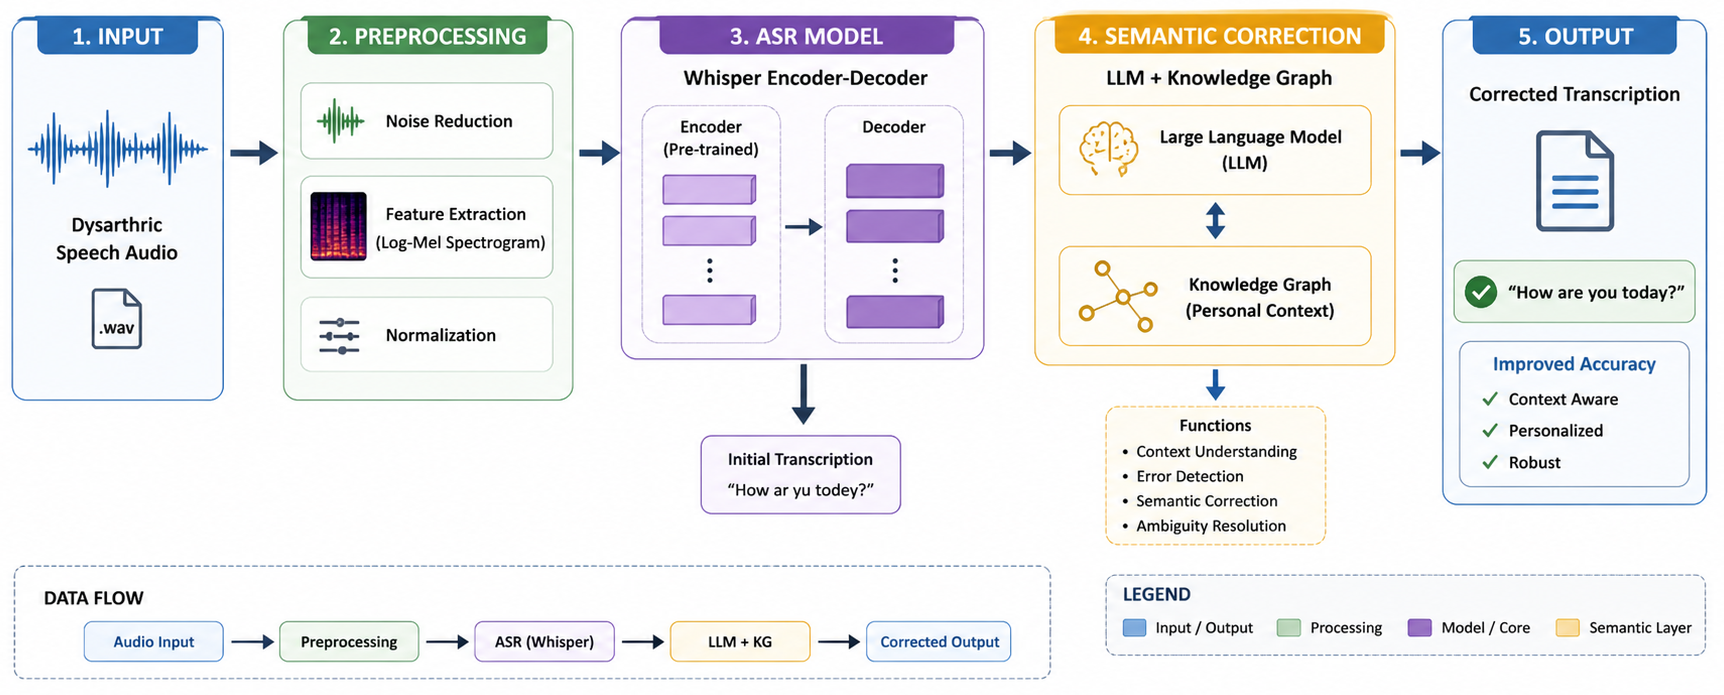
\includegraphics[width=0.9\textwidth]{Figures/architecture_block_diagram.png}
	\caption{Intelligent Fault Detection System Architecture}
	\label{fig:architecture}
\end{figure}

\section{Performance Evaluation}
After integrating all system components, the system is evaluated under simulated real-time conditions.

The results indicate:
\begin{itemize}
\item High accuracy in fault detection and classification
\item Low latency suitable for real-time applications
\item Effective identification of high-risk fault scenarios
\item Improved operator understanding through AI-generated insights
\end{itemize}

The integration of decision intelligence and AI significantly enhances the overall effectiveness of the system compared to traditional approaches.

\section{Summary}
The implementation presents a comprehensive pipeline for intelligent fault detection and predictive governance. Starting from real-time sensor data acquisition, the system performs embedded fault classification, followed by decision intelligence analysis and AI-based interpretation. The smart governance layer automates system responses, ensuring efficient fault management. The combined approach results in improved detection speed, better decision-making, and enhanced operational reliability. The next chapter focuses on detailed analysis and comparison of results obtained from different configurations and experiments.